\chapter{Extending Adaptively Restrained Particle Simulation to Graphical Simulations}
\label{chap:arps}

\begin{figure}[!h]
    \begin{tabular}{cc}
        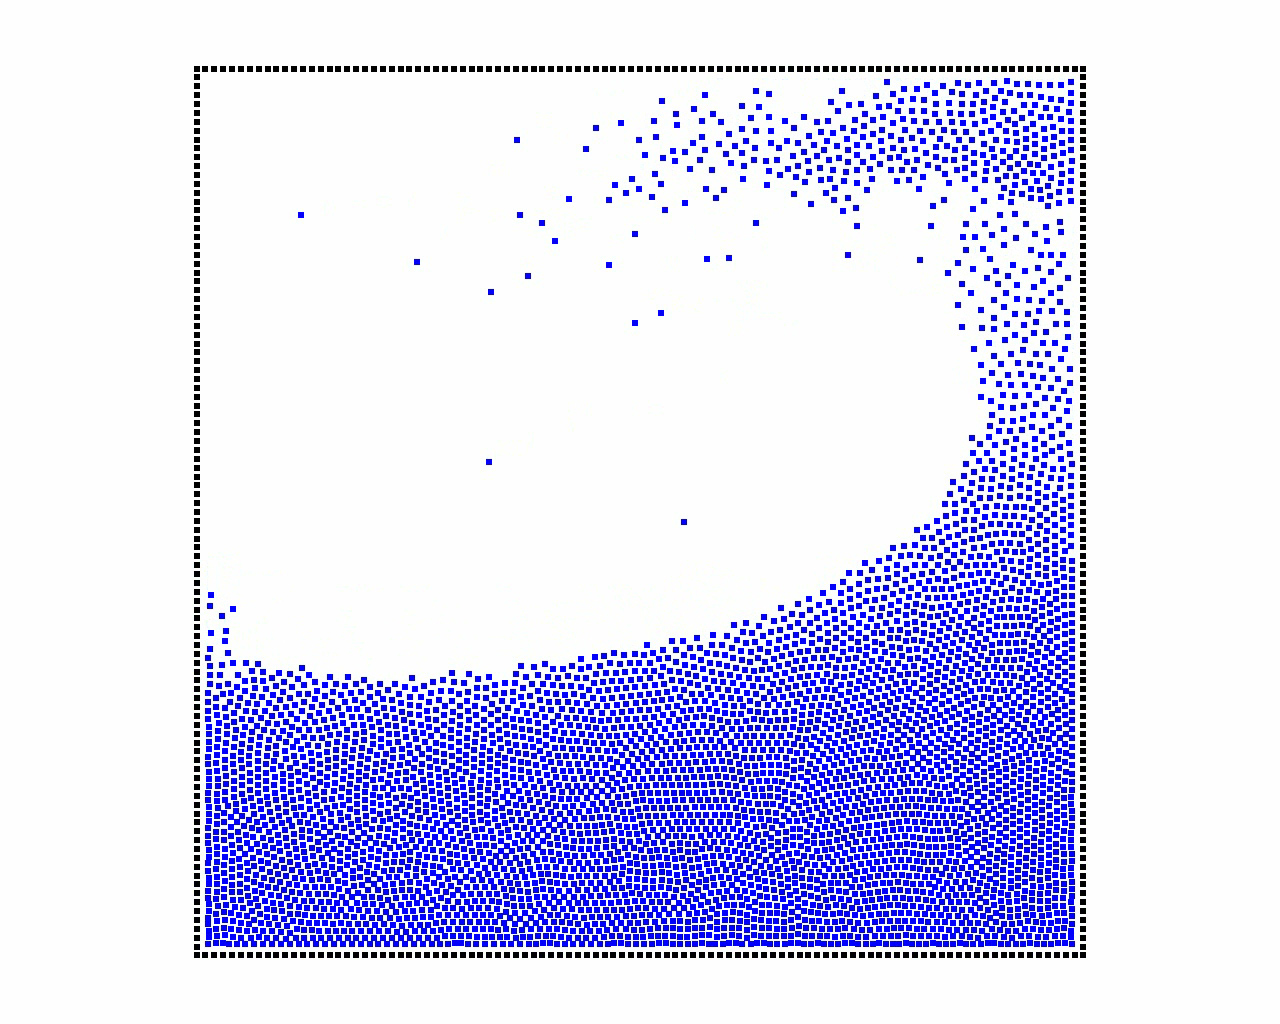
\includegraphics[width=0.4\linewidth]{images/arps-vriphys2013/ReposSPHClassique1.jpg} &
        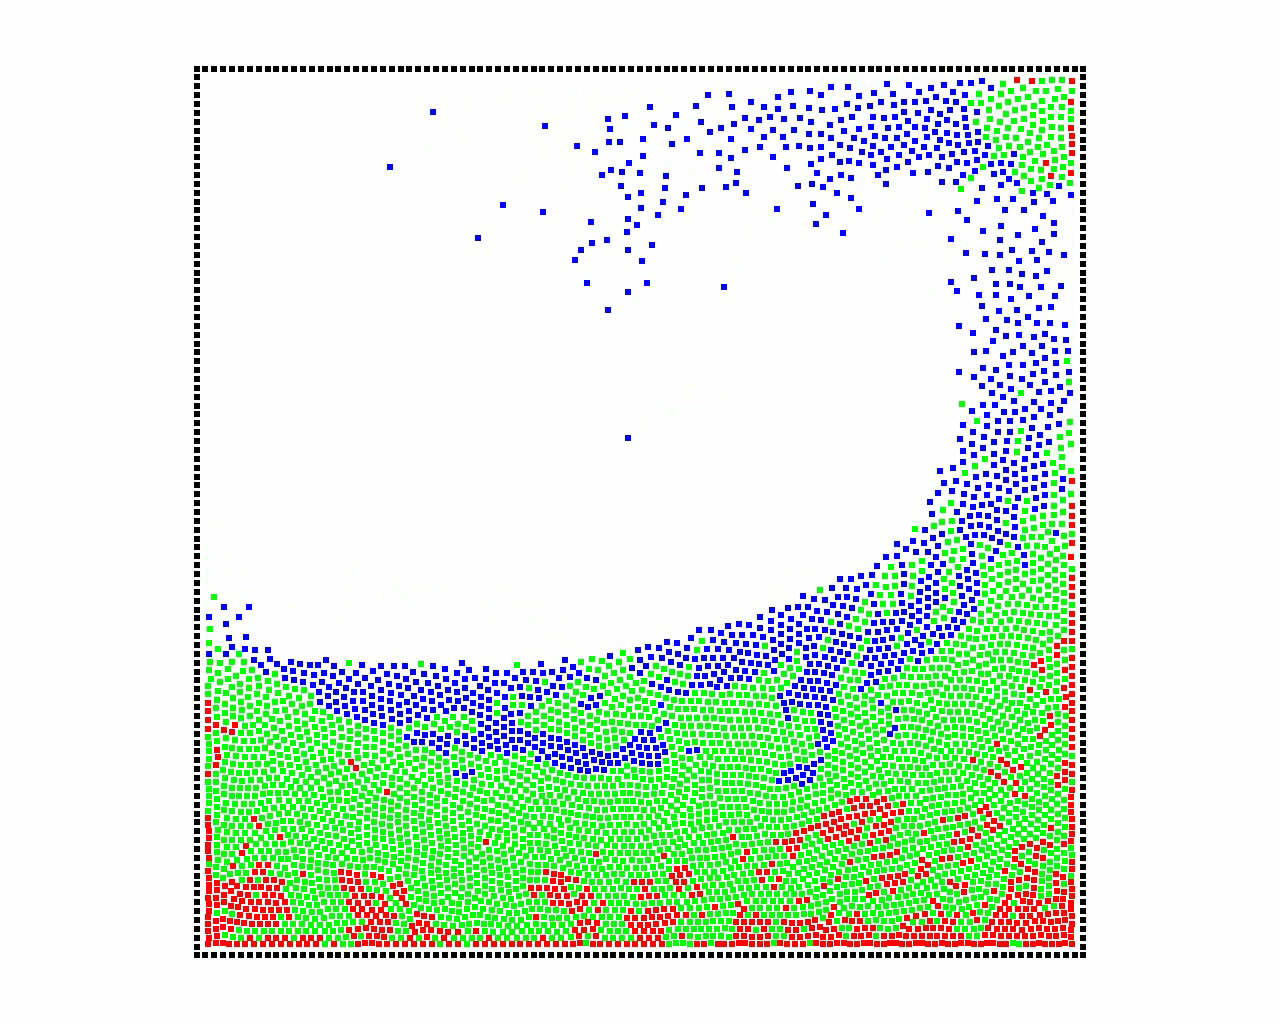
\includegraphics[width=0.4\linewidth]{images/arps-vriphys2013/ReposSPHARPSColor1.jpg}
    \end{tabular}
 \centering
 \caption[ARPS: Dam break simulations]{ A dam break simulation with 5000 particles simulated with WCSPH (on the left)
 and with our adaptive method (on the right). On the right image, blue corresponds to full-dynamics particles, green to transition particles and red to restrained particles.}
\label{fig:ARPS_Teaser}
\end{figure}

Combining efficiency with visual realism had been one of the main goals of Computer Graphics research in the last decade. As presented in Section~\ref{sec:starAdaptivity}, the general strategy for efficient graphical simulations is to concentrate the computational time on the most interesting parts of an animated scene (such as near the surface of a fluid), while simplifying the rest of the scene according to some visual quality criteria.  A number of adaptive simulation methods, aimed at controlling the trade-off between performance and precision, have been developed. Most of them consist in changing time or space sampling, using adaptive time steps or multi-scale models.
Although several of them give impressive results, they are often difficult to implement, they may be restricted to specific applications and they sometimes generate discontinuity artifacts due to sudden simplifications.
\\ \\
A different approach for adaptive simulation~\cite{Artemova2012} was proposed in the context of molecular dynamics~(MD). Contrary to the Computer Graphics methods reviewed in Section~\ref{sec:starAdaptivity}, Adaptively Restrained Particle Simulations (ARPS) do not adapt time or space sampling, but rather switch the positional degrees of freedom of particles on and off, while letting their momenta evolve. The key idea is that since most of the computation time is spent in computing interaction forces based on positions, particles with low velocity could be considered fixed in space - and the corresponding interaction forces constant - until they accumulate enough momentum to start moving again. Therefore, inter-particles forces do not have to be updated at each time step, in contrast with traditional methods that spend a lot of time there.
\\ \\
While freezing objects to gain computation time has been extensively used in video games, the question of when and how to release them has not been extensively studied, and has mainly relied on \textit{ad hoc} heuristics.
Adaptively Restrained Particle Simulations~(ARPS), in contrast, introduce a physically sound approach with proven correctness, and has been successfully used in the context of predictive, energy- and momentum-conserving particle simulation.
\\ \\
In this chapter, we explore the use of Adaptively Restrained (AR) particles for graphics simulations. Our experiments show that this new, simple strategy for adaptive simulations can provide significant speedups more easily than traditional adaptive models. The key contributions of our work are as follows: 
\begin{itemize}
\item We adapt ARPS to particle-based fluid simulations and propose an efficient incremental algorithm to update forces and scalar fields in Section~\ref{sec:arps_sph}.
\item We introduce a new implicit integration scheme enabling to use ARPS for stiff objects simulation such as cloth simulation in Section~\ref{sec:arps_implicit}.
\end{itemize}
The remainder of this chapter is organized as follows: 
Section~\ref{sec:arps_basics} presents the initial formulation of ARPS that was introduced for molecular dynamics simulations and explores its potential for Computer Graphics applications. 
Section~\ref{sec:arps_sph} and \ref{sec:arps_implicit} respectively introduce our extension of ARPS to fluid and stiff objects simulations. 
Section~\ref{sec:arps_implementation} deals with the practical implementation and parameters tuning. 
Section~\ref{sec:arps_discussion} concludes and gives some perspectives of future works.

%-------------------------------------------------------------------------
\section{Adaptively Restrained Particles} 
\label{sec:arps_basics}
%-------------------------------------------------------------------------
\paragraph*{Basic ideas:}
Adaptively Restrained Particle Simulations (ARPS)~\cite{Artemova2012} was recently developed to speed up particle simulations in the field of Molecular Dynamics.
They rely on Hamiltonian mechanics, where the state of a particle system is described by a position vector $\vec q$ and a momentum vector $\vec p$, and its time evolution is governed by the following differential equations:
\begin{eqnarray*}
\frac{d\vp}{dt} &=& -\frac{\partial \H}{\partial \vq} \\
\frac{d\vq}{dt} &=& +\frac{\partial \H}{\partial \vp}
\end{eqnarray*}
Here, the Hamiltonian $\H$ is the total mechanical energy given by:
\begin{equation}
    \label{eq:hamiltonian}
    \H(\vq,\vp) = \frac{1}{2} \vp^{T}M^{-1}\vp + V(\vq)
\end{equation}
where the first term corresponds to the kinetic energy, while the second represents the potential energy.
In \cite{Artemova2012}, an \textit{adaptively restrained} (AR) Hamiltonian is introduced:
\begin{equation}
    \label{eq:arhamiltonian}
    \H_{AR}(\vq, \vp) = \frac{1}{2} \vp^{T}\Phi(\vq,\vp)\vp + V(\vq)
\end{equation}
The matrix $\Phi$ is a block-diagonal matrix used to switch on or off the positional degrees of freedom of the particles during the simulation.
Each $3$x$3$ block corresponds to a particle $i$ and is equal to
$\Phi_{i}(q_{i}, p_{i}) = m_{i}^{-1}[1 - \rho_{i}(q_{i}, p_{i})]\mathbf{I_{3\mathtt{x}3}}$.
The function $\rho_{i} \in [0, 1]$ is called the \emph{restraining function}.
When $\rho_{i} = 0$, $\Phi_{i} = m_{i}^{-1}$ and the particle is \textit{active}: it obeys standard (full) dynamics.
When $\rho_{i} = 1$, $\Phi_{i} = 0$ and the particle is \textit{inactive} (not moving). When $\rho_{i} \in [0, 1]$, the particle is in transition between the two states.
%-------------------------------------------------------------------------
The restraining function $\rho_{i}$ of each particle is used to decide \emph{when} to switch positional degrees of freedom on or off.
In \cite{Artemova2012}, $\rho_{i}$ depends on the particle kinetic energy.
The function uses two thresholds, a restrained-dynamics threshold $\epsilon^{r}$ and a full-dynamics threshold $\epsilon^{f}$.
It is defined as :
\begin{equation}
    \label{eq:restrainingfunction}
    \rho_{i}(p_{i}) =
    \displaystyle\left\lbrace
    \begin{array}{lccc}
        1, & & & \textrm{if } 0 \leq K_{i}(p_{i}) \leq \epsilon_{i}^{r} \\
        0, & & & \textrm{if } K_{i}(p_{i}) \geq \epsilon_{i}^{f} \\
        s(K_{i}(p_{i})) \in [0, 1], & & & \textrm{elsewhere} \\
    \end{array}
    \right.
\end{equation}
where $K_i=p_i^2/2m_i$ is the kinetic energy, and
$s$ is a twice-differentiable function. In practice a $5^{th}$-order spline is used.
%-------------------------------------------------------------------------
\paragraph*{Adaptive equations of motion:}
The adaptive equations of motions are derived from the AR Hamiltonian (\ref{eq:arhamiltonian}):
\begin{equation}
   \label{eq::armotionequation}
    \displaystyle
    \begin{array}{l}
        \displaystyle \frac{d\vp}{dt} =
        -\frac{\partial \H_{AR}}{\partial \vq} = -\frac{\partial V(\vq)}{\partial \vq} \\ \\
        \displaystyle \frac{d\vq}{dt} =
       \frac{\partial \H_{AR}}{\partial \vp} = M^{-1}[I - \rho(\vp)] \vp
        - \frac{1}{2}\vp^{T}M^{-1}\frac{\partial \rho(\vp)}{\partial \vp}\vp\\
    \end{array}
\end{equation}
Applied to a particle, one can derive the rate of position change, which we call \textit{effective velocity}, as:
\begin{equation}
    \label{eq:adaptiveVelocity}
    \dot{q}^{eff} = \frac{1}{m}\left((1-\rho(p))p - \frac{1}{2}\parallel p \parallel^2\frac{\partial \rho(p)}{\partial p}\right)
\end{equation}
While the momenta evolve as in classical Hamiltonian mechanics, the position evolve differently.
When a particle's momentum is small enough, the particle becomes inactive and stops moving.
However, even if the particle is inactive, its momentum may change.
Therefore its kinetic energy may become large enough again for the particle to resume moving.
In general, particles switch between active and inactive states during the simulation.
%-------------------------------------------------------------------------
\begin{figure}[htb]
  \centering
  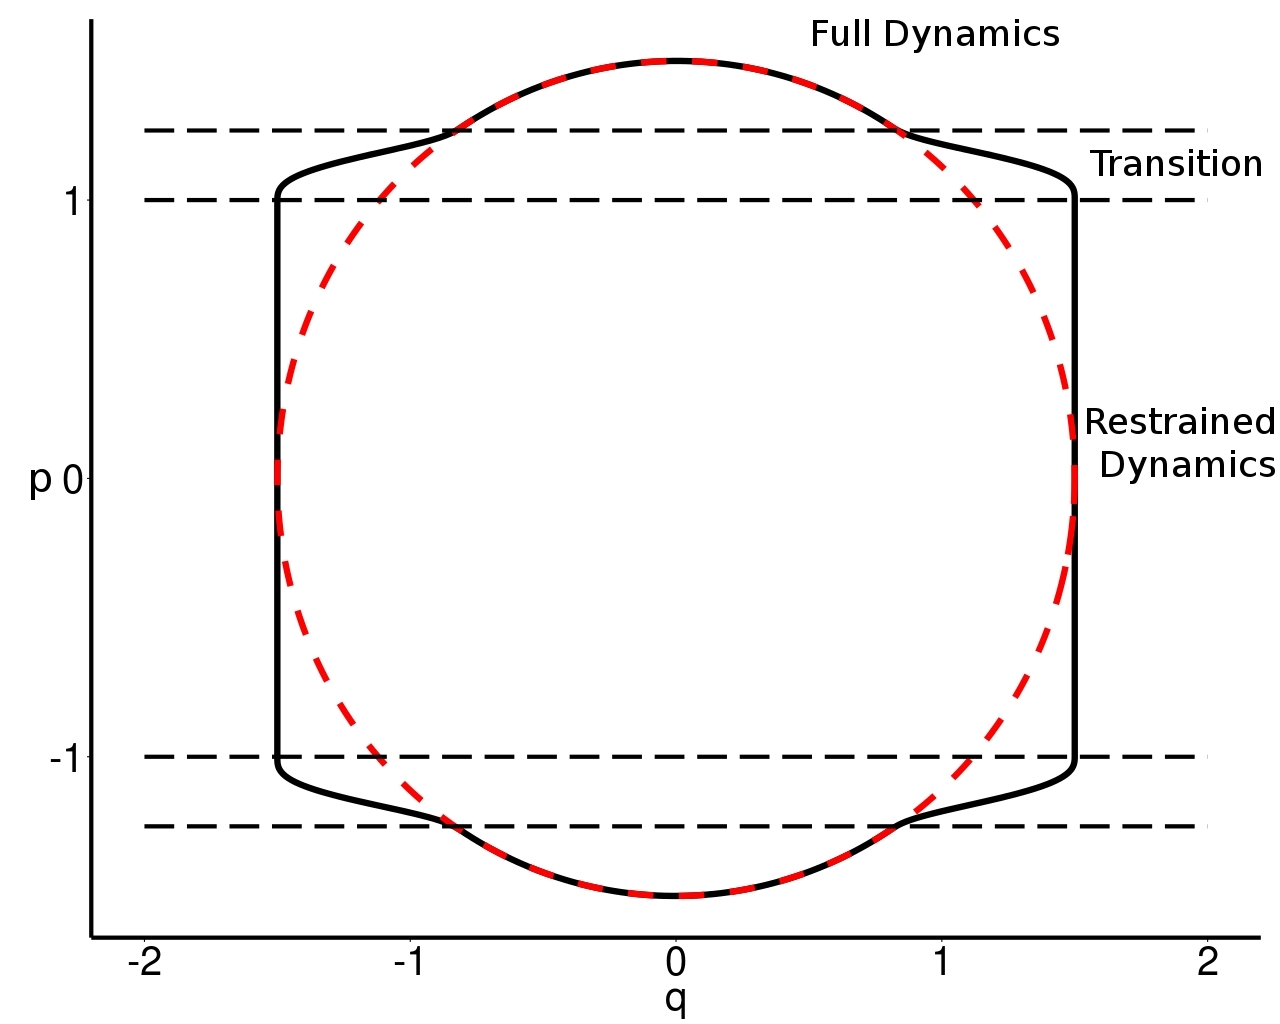
\includegraphics[width=0.8\linewidth]{images/arps-vriphys2013/harmonicOscillatorPhasePortraitraw.jpeg}
  \caption[ARPS: Phase portrait of a ARPS harmonic oscillator]{\label{fig:harmonicOscillatorPhasePortrait} Phase portrait of a harmonic oscillator. The red dotted ellipse corresponds to standard Hamiltonian mechanics, while the solid black line corresponds to ARPS. During restrained dynamics, the particle's momentum is accumulated. When enough energy has been accumulated, a transition phase takes place leading the particle to switch back to full dynamics.}
\end{figure}

\paragraph*{A simple example:}
Consider a 1D harmonic oscillator : a particle attached to the origin with a perfect spring.
Fig. \ref{fig:harmonicOscillatorPhasePortrait} shows a phase portrait of the corresponding
AR system.
In classical mechanics, the trajectory of the state in this (position, momentum) space is an ellipse, the size of which depends on the (constant) energy of the system.
Using ARPS, the position is constant (vertical straight parts) as long as the kinetic energy is small enough, while it is an ellipse as long as the kinetic energy is big enough.
These trajectories are connected by a transition corresponding to an energy between the two thersholds of eq.~(\ref{eq:restrainingfunction}).
The closed trajectory corresponds to a constant \textit{adaptively restrained energy} $H_{AR}$.

\begin{figure}[ht!]
  \centering
  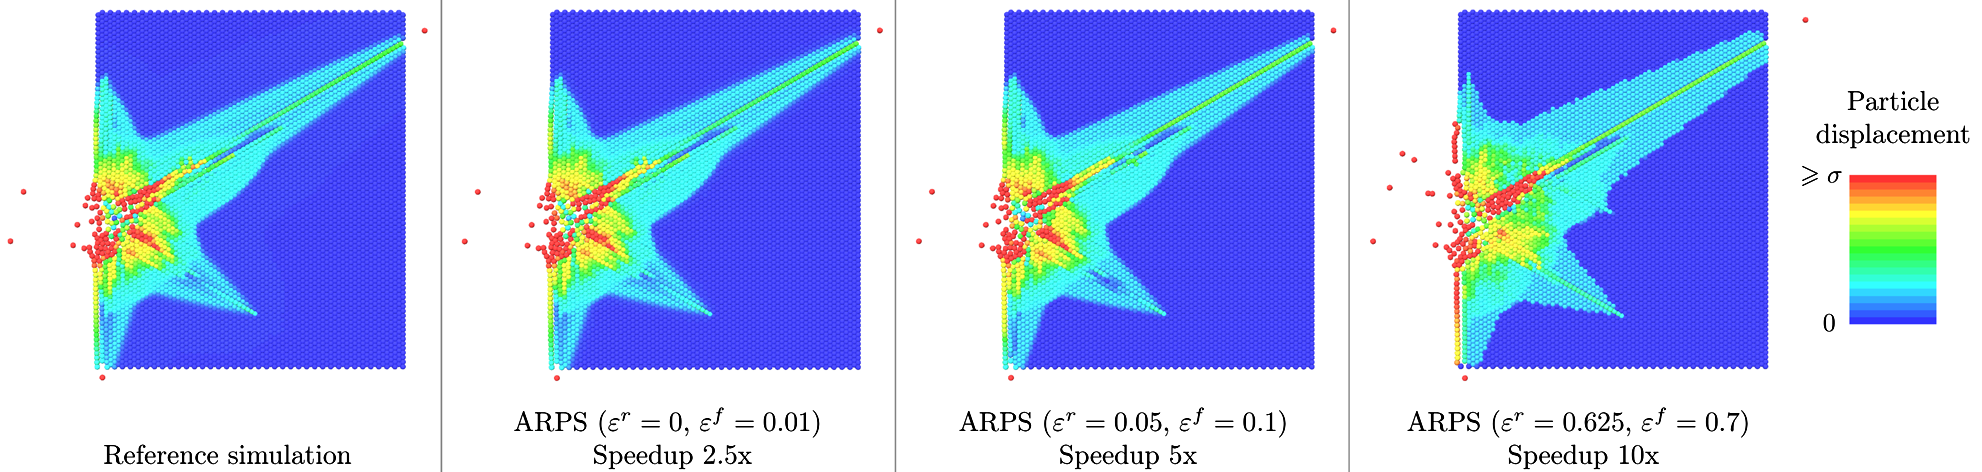
\includegraphics[width=1.0\linewidth]{images/arps-vriphys2013/ARPS_Collision_Artemova.png}
  \caption[ARPS: Collision Cascade from \cite{Artemova2012}]{\label{fig:cascadeCollision} 
      A particle is launched at high velocity toward a 2D static particle system made of $5390$ particles, resulting into a collision cascade~\cite{Artemova2012}. 
 On the left, the result of a full dynamics simulation. 
 The three other images are the result of ARPS with different thresholds which allow to obtain a smooth trade between efficiency and precision.}
\end{figure}

\paragraph*{Generalization:}
Due to the similarity of the adaptive kinetic energy with the standard kinetic energy, particle systems simulated using ARPS exhibit the expected properties of standard physical simulation, namely the conservation of momentum and (adaptive) energy. It is therefore possible to perform macroscopically realistic simulations with reduced computation time as illustrated in Figure~\ref{fig:cascadeCollision}.

%-------------------------------------------------------------------------
\paragraph*{Computational performance:}
The authors of \cite{Artemova2012}, Artemova and Redon obtained significant speed-ups by exploiting the immobility of particles. Figure~\ref{fig:cascadeCollision} illustrates one of their result where a $10\times$ speed-up was achieved in a collision scenario while keeping a behavior close to the reference one. In this example, inter-particles forces were derived from a Lennard-Jones potential. To save time on inactive particles, they proposed an incremental method to update the particles' forces at each time step:
\begin{enumerate}
    \item All forces that were acting on each active particle at the previous time step are substracted based on previous position.
    \item New forces based on current positions are added to each active particle.
\end{enumerate}
The increase of computational performance comes from the absence of force computation between
two inactive particles and the absence of neighbor search for inactive particles.
As these two steps are common bottlenecks in particle simulation, significant speedup can be achieved.

%-------------------------------------------------------------------------
\paragraph*{Potential benefits of extension to Computer Graphics:}
Molecular dynamics often inspired particle-based simulations in Computer Graphics. The same bottleneck, namely inter-particles forces computation based on neighbor search, is present in the two fields, so we can expect interesting performance for ARPS in graphics. The remainder of this chapter explores two applications of ARPS to graphical simulations:
\begin{enumerate}
\item Particle-based fluid simulation. Originally, ARPS has been applied to conservative system. While fluid simulation involves position-based forces, it also involves velocity-based damping forces that need to be taken care of. We propose a simple method to handle them. Additionnaly, we extend the incremental algorithm proposed by Artemova and Redon to update forces as well as scalar fields.
\item Stiff object simulation. Explicit integration of stiff objects such as cloth is expensive due to stability issues. A well known solution is to use implicit integration instead. We derive an implicit formulation of ARPS and propose a hybrid solver to exploit the inactivity of particles in cloth simulation.
\end{enumerate}
It is clear that ARPS is not well-suited for simulations where all degree of freedom move: classical spatial adaptation is better suited in this case. In contrast, ARPS is best suited for simulations where most parts are immobile but may resume moving at any time. Even if these situations are not the most visually exciting, they are very common in Computer Graphics: they include simulation of characters clothing when many of the characters are at rest, surgical simulations with local-only user interaction, and the animation of large volumes of liquid, when most of it already came to rest.

%-------------------------------------------------------------------------
\section{ Extension to SPH fluid simulation } 
\label{sec:arps_sph}
As presented in section~\ref{subsubsec:starSPH}, SPH fluid simulation is widely used in computer graphics and many methods have been proposed \cite{Desbrun1996}, \cite{Muller2003}, \cite{Solenthaler2009}, \cite{Ihmsen2014:IISPH}.
SPH approximates fluid dynamics with a set of particles.
The particles are used to interpolate the properties of the fluid anywhere in space.
Each particle samples the fluid properties such as density, pressure or temperature. All these properties are updated based on the particle neighbors and are
used in short-ranged inter-particle forces.
To integrate ARPS, we chose WCSPH (Weakly Compressible Smoothed Particle Simulation) \cite{Becker2007WCSPH}, a standard SPH formulation \cite{Desbrun1996}, \cite{Muller2003}. For the sake of simplicity, we limit our discussion to the main inter-particles forces: pressure and viscosity. 
\begin{algorithm}[H]
    \caption[ARPS: WCSPH simulation]{WCSPH simulation loop}
    \label{alg:WCSPH}
    \begin{algorithmic}
	\ForAll{particle $i$}
	    \State find neighbors $j$
    \EndFor
    \ForAll{particle $i$}
    \State compute $\rho_{i}$ (e.g. Eq.~\ref{eq:densitySPH})
    \State compute $p_{i}$ using $\rho_{i}$ (e.g. Eq.~\ref{eq:pressureSPH})
    \EndFor
    \ForAll{particle $i$}
    \State $\displaystyle \mathbf{f}_{i}^{pressure} = -\frac{m_{i}}{\rho_{i}}\nabla p_{i}$ (e.g. Eq.~\ref{eq:pressureGradientSPH})
    \State $\displaystyle \mathbf{f}_{i}^{viscosity} = m_{i}\eta\nabla^{2}\mathbf{v}_{i}$ (e.g. Eq.~\ref{eq:velocityLaplacianSPH})
    \State $\displaystyle \mathbf{f}_{i}(t) = \mathbf{f}_{i}^{pressure} + \mathbf{f}_{i}^{viscosity} + \mathbf{f}_{i}^{other}$
    \EndFor
    \ForAll{particle $i$}
    \State $\mathbf{v}_{i}(t+\Delta t) = \mathbf{v}_{i}(t) + \Delta t \mathbf{f}_{i}(t)/m_{i}$
    \State $\mathbf{x}_{i}(t+\Delta t) = \mathbf{x}_{i}(t) + \Delta t \mathbf{v}_{i}(t+\Delta t)$
    \EndFor
    \end{algorithmic}
\end{algorithm}
ARPS can save time on each computation step involving the position of the particles.
In SPH fluid simulation, every property of a particle is computed as a weighted sum of its neighbors' property.
And the weights are computed based on the position of the particle and its neighbors.
Therefore, time can be saved as soon as a particle is close to immobility. 
This makes SPH a perfect candidate for ARPS.
\\ \\
As long as a particle is inactive and is surrounded by inactive particles, its properties and neighborhood do not need to be updated.
In practice, this includes pressure and viscosity forces as well as density and pressure scalar field.
\\ \\
To gain computational time from the inactive particles, we extend the incremental algorithm proposed in \cite{Artemova2012} (see Algorithm~\ref{alg:WCSPHARPS}).
In this algorithm we denote as \emph{active} every \emph{active} or {transitive} particle.
From one step to another, all the contributions to physical properties from active particles are updated. 
Thus, even inactive particles whose neighbors are active are kept up-to-date.
\begin{algorithm}[H]
    \caption[ARPS: WCSPH+ARPS simulation]{WCSPH+ARPS simulation loop}
    \label{alg:WCSPHARPS}
    \begin{algorithmic}
        \If{step=1}
        \State Perform Algorithm~\ref{alg:WCSPH}
        \Else
            \ForAll{\textbf{active} particle and its neighbors $i$}
            \State Substract old density contribution from neighbor $j$
	        \State Subtract old pressure/viscosity force contribution from neighbor $j$
            \EndFor
            \ForAll{\textbf{active} particle neighbors $i$}
            \State find neighbors $j$
            \EndFor
            \ForAll{\textbf{active} particle and its neighbors $i$}
            \State Add new density contribution from neighbor $j$
            \State Update pressure $p_{i}$
	        \State Add new pressure/viscosity force contribution from neighbor $j$
            \State Add new density contribution from neighbor $j$
            \EndFor
            \ForAll{particle $i$}
            \State $\mathbf{v}_{i}(t+\Delta t) = \mathbf{v}_{i}(t) + \Delta t \mathbf{f}_{i}(t)/m_{i}$
            \State $\mathbf{x}_{i}(t+\Delta t) = \mathbf{x}_{i}(t) + \Delta t \mathbf{q}^{eff}_{i}(t+\Delta t)$
            \State Update particle's state based on $\rho(p)$.
            \EndFor
        \EndIf
    \end{algorithmic}
\end{algorithm}
%-------------------------------------------------------------------------------
\subsection{Viscosity}
Viscosity forces involve particles velocities. The viscosity force of particle $i$ with respect to particle $j$ is :
\begin{equation}
	\label{eq:viscosityForces}
	f_{ij} =
	\left\lbrace	
	\begin{array}{lrr}
	-m_{i}m_{j}\Pi_{ij}\nabla W_{ij} & & v_{ij}^{T}q_{ij}<0\\
	& & \\
	0 & & v_{ij}^{T}q_{ij} \geq 0 \\
	\end{array}		
	\right.
\end{equation}
$\Pi_{ij}$ is given as :
\begin{equation}
\label{eq:pij}
	\Pi_{ij} = -\nu\left( \frac{v_{ij}^{T}q_{ij}}{ \mid q_{ij} \mid^{2} + \epsilon h^{2} } \right)
\end{equation}
$W_{ij}$ denotes a convolution kernel, $v_{ij}$ the difference of velocities between the two particles, $q_{ij}$ the difference of positions between the two particles, $m_{i}$ is the mass, $h$ is the particle smoothing radius and $\nu = \frac{2 \alpha h c_{s}}{ d_{i} + d_{j} }$ is a viscous term where $\alpha$ is a viscosity constant,
$d_{i}$ the particle $i$ density.
$\epsilon=0.01$ is a constant to avoid singularities.
\newline \newline
However, velocity is not explictly represented in ARPS, and can be seen in two different ways. We may define it based on the momentum and set $ v_{i} = p_{i} / m_{i} $, or based on the change of position $  \dot{q}_{i}$.
In the first case, we can get time-varying forces even for inactive particles, which we want to avoid.
We therefore use the effective velocity of the particle, as defined in eq.(\ref{eq:adaptiveVelocity}).
Applied to a harmonic oscillator, this results in the behavior illustrated in Fig. \ref{fig:HODampedPP}.
The more the particle is damped the longer it remains inactive, which is an intuitive behavior.
%%% HARMONIC OSCILLATOR DAMPED%%%
\begin{figure}[htb]
  \centering
  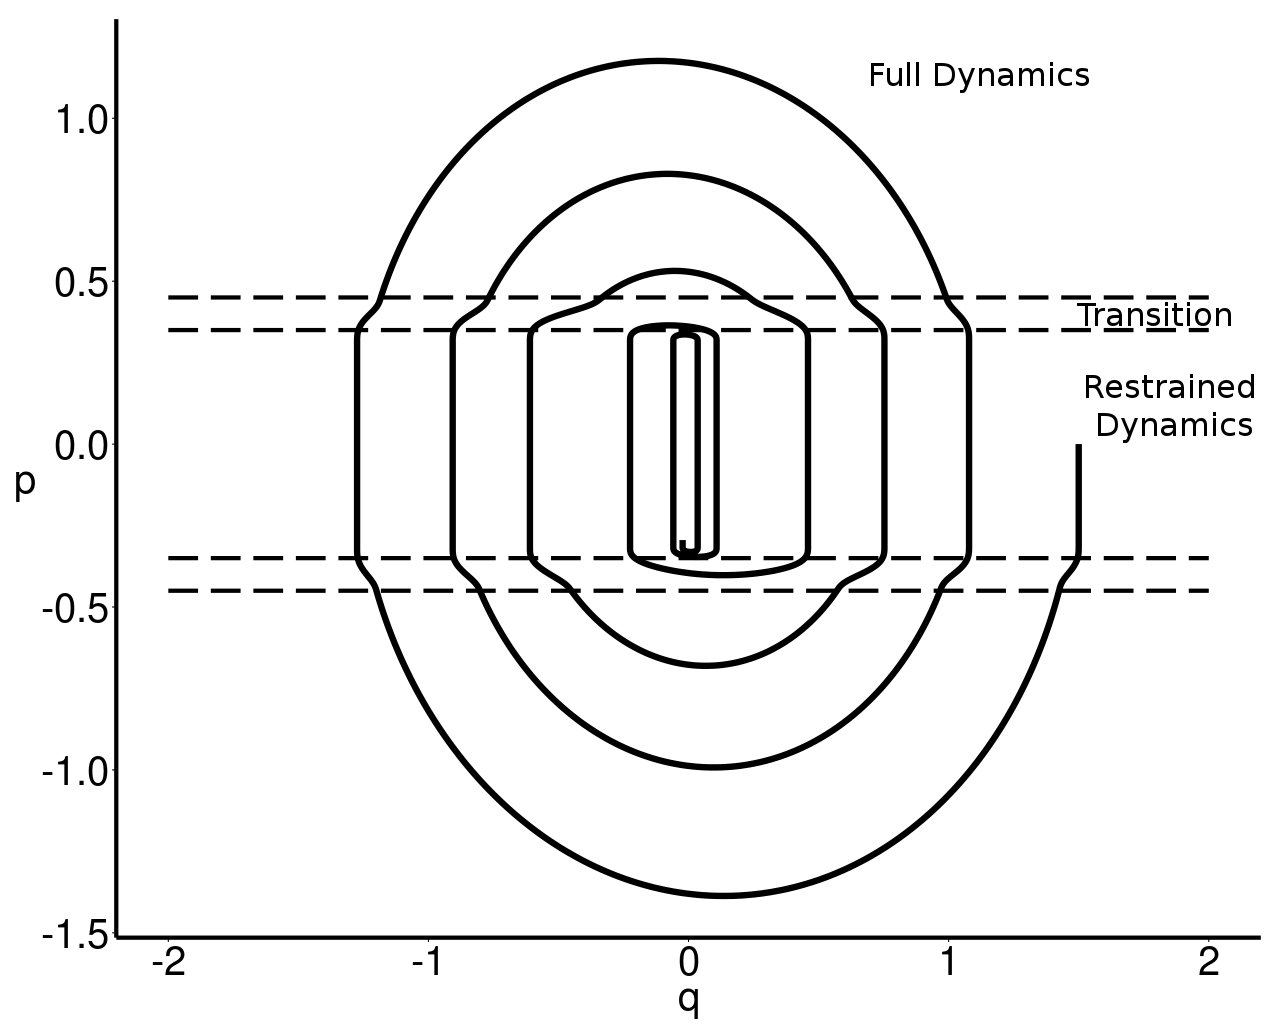
\includegraphics[width=0.8\linewidth]{images/arps-vriphys2013/harmonicOscillatorDampedPhasePortraitraw.jpeg}
  \caption[ARPS: Phase portrait of a damped ARPS harmonic oscillator]{\label{fig:HODampedPP} Phase portrait of our damping approach in ARPS.
  As with a classic damped oscillator we obtain a spiral phase portrait.}
\end{figure}
%-------------------------------------------------------------------------
\subsection{Modified inactivity criterion}
Since our damping force vanishes along with the effective velocity of the particle, it drags down the kinetic energy asymptotically close to the inactivity threshold, without ever reaching it.
Consequently, particles only subject to damping forces never become inactive, and we do not spare computation time, even when the particles get nearly static.
To remedy this problem, we consider inactive the particles which effective velocity fall below a user-defined threshold.
%-------------------------------------------------------------------------
\subsection{Performance}
We performed two experiments to measure computation time.
The first one (Table~\ref{table:perf1}) is a fall of $5000$ particles in a box.
As soon as most particles come to rest, and become inactive the speedup can be significant.
For $15$s, the mean speedup is $3.8$.
The speedup can locally reach $25.7$.
\begin{table}[htb]
   \centering
\begin{tabular}{|c|c|c|c|} \hline
    Simulation Time & SPH   & ARPS    & Speed-up \\ \hline
    15s     & 893s   & 232s                 &  \{0.91, 25.73, 3.85\}\\ \hline
\end{tabular}
\caption[ARPS: Fall of a block of water - Measurements]{\label{table:perf1}Fall of a block of water - Computation time and speedup \{min, max, mean\}}
\end{table}
We can see in Figure~\ref{fig:ARPS_Teaser} that during speed movements most of the particles are active so that the adaptive simulation stay close to reference simulation.
Therefore small scale details like splashes can be preserved.
\begin{figure*}[!ht]
    \centering
    \begin{tabular}{ccc}
        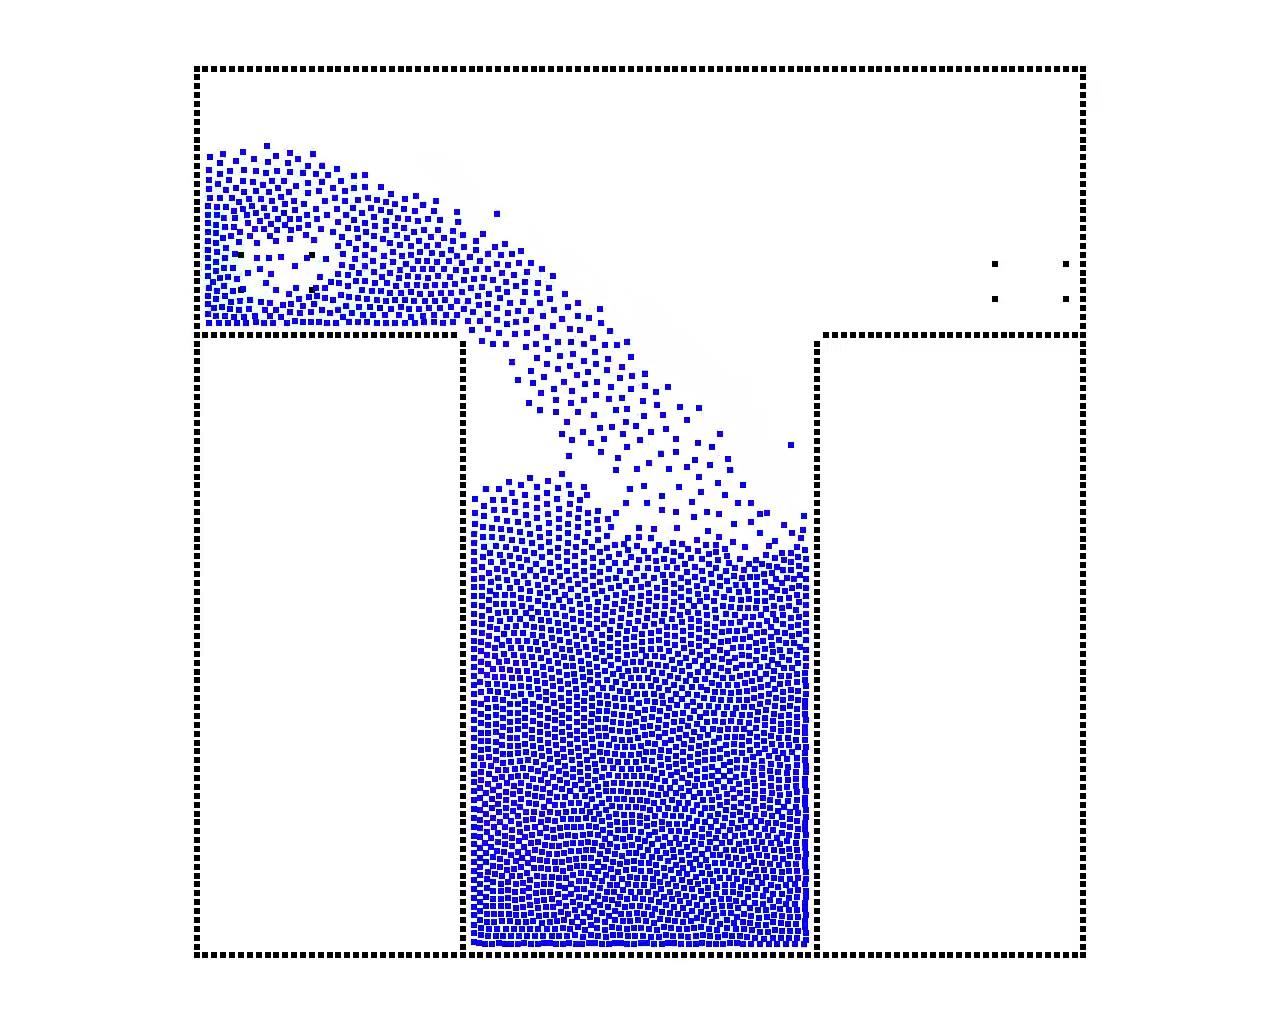
\includegraphics[width=.32\linewidth]{images/arps-vriphys2013/PermanentFlowSPH.jpg} &
        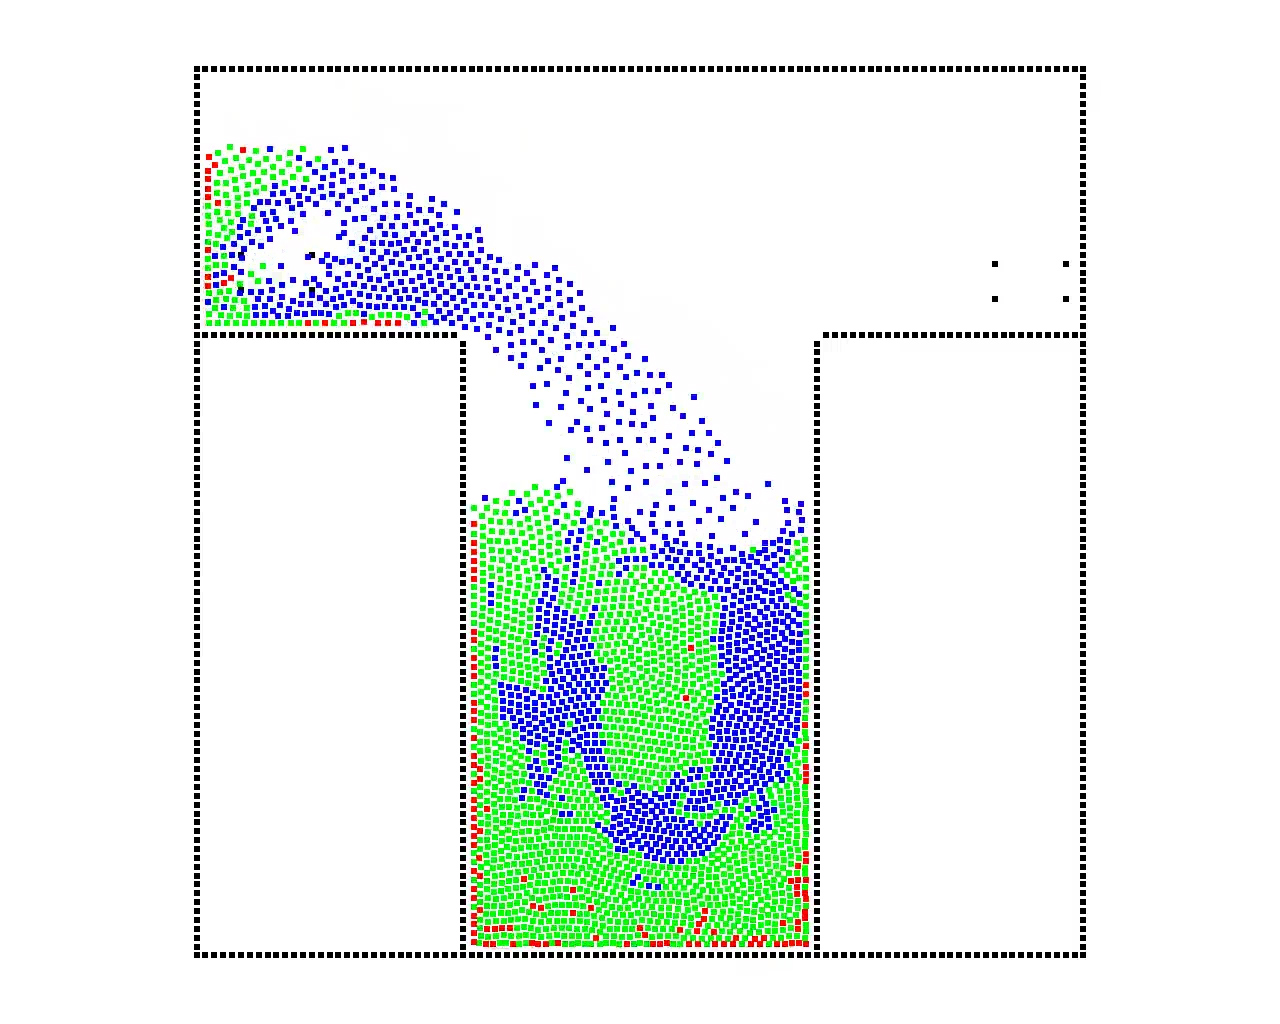
\includegraphics[width=.32\linewidth]{images/arps-vriphys2013/PermanentFlowARPSColor.jpg} &
  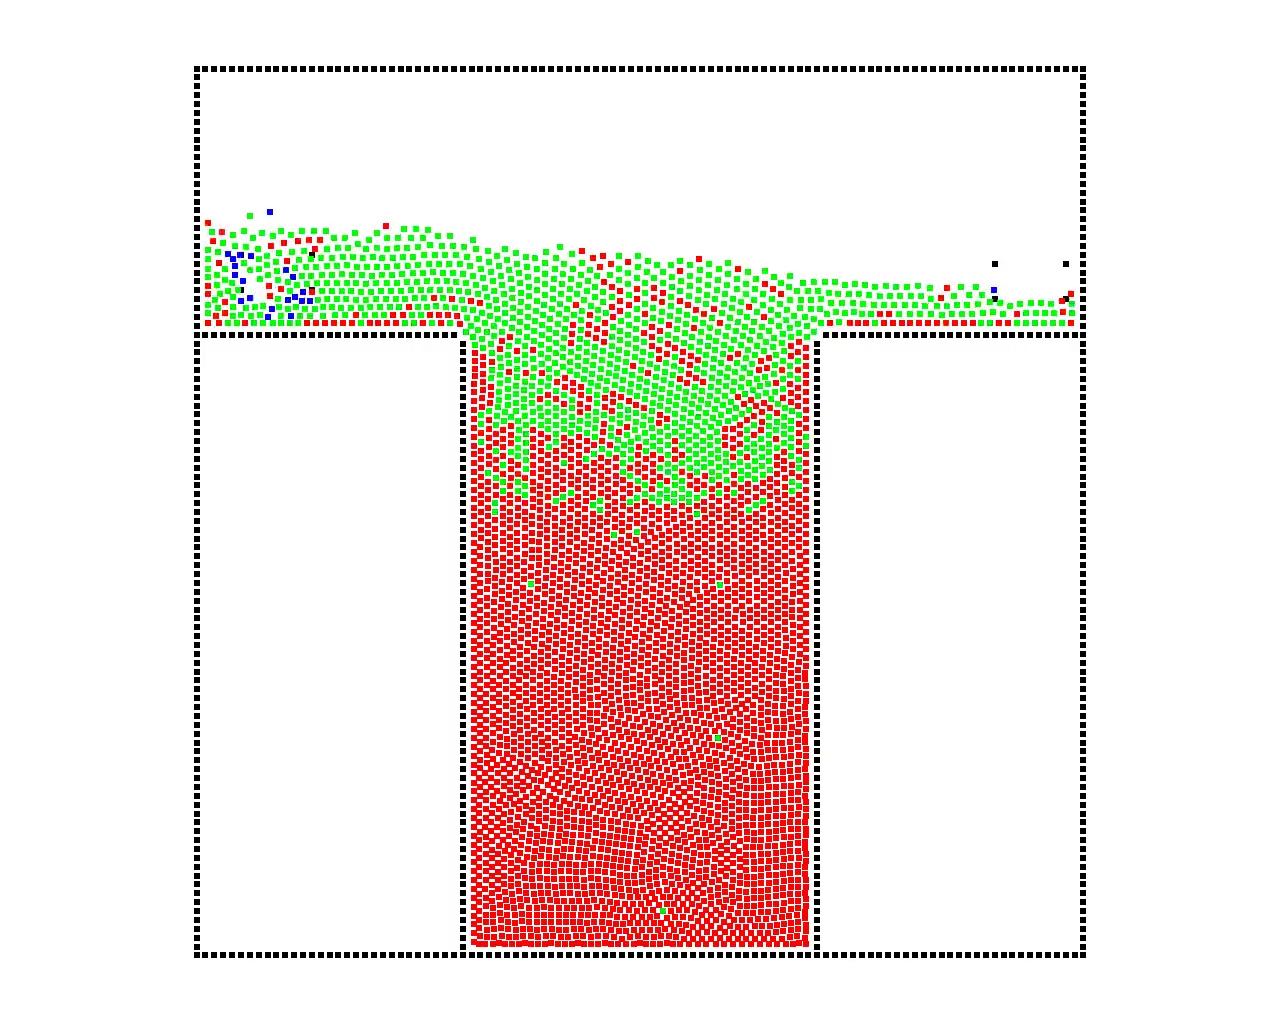
\includegraphics[width=.32\linewidth]{images/arps-vriphys2013/PermanentFlowARPSColor2.jpg} \\
  (a) & (b) & (c)
    \end{tabular}
    \caption[ARPS: Permanent flow simulations]{\label{fig:permanentflow} A permanent flow simulation with 4240 particles.
    (a) is a classic WCSPH simulation. (b) is our adaptive method at the same time of (a) with restrained particles in red. (c) is our adaptive method once the permanent flow is installed.}
\end{figure*}
\newline
The second experiment (see Table~\ref{table:perf2}) is the creation of a permanent flow with $4240$ particles. As we can see in Figure~\ref{fig:permanentflow}, once the permanent flow is installed a large amount of particles are restrained. We reach an interesting speedup while keeping a motion close to the reference.
\begin{table}[htb]
    \centering
\begin{tabular}{|c|c|c|c|} \hline
    Simulation Time & SPH       & ARPS    & Speed-up \\ \hline
    30s         & 2166s     & 814s              & \{0.83, 3.99, 2.66\} \\ \hline
\end{tabular}
\caption[ARPS: Fluid permanent flow - Measurements]{\label{table:perf2}Fluid permanent flow - Computation time and speedup \{min, max, mean\}.}
\end{table}
%-------------------------------------------------------------------------
\section{Extension to stiff objects: Implicit Integration} 
\label{sec:arps_implicit}
In this section we explore the application of ARPS to stiff object simulation and propose an implicit integration scheme which saves computation time for particles at rest.
Implicit integration for cloth simulation was introduced in \cite{Baraff1998}. An introduction to implicit integration is proposed in \cite{Witkin2001}.
While originally formulated on velocity, it can be straightforwardly expressed on momentum.
Instead of integrating the momentum using the forces at the current time step, implicit integration uses the forces at the end of the current step.
As we do not know these forces we end up with a non linear function and after linearization with a linear system to solve to obtain the next momentum:
\begin{equation}
    \label{eq:implicit}
    ( I -h^{2}KM^{-1} ) \Delta p = h( f + h KM^{-1}p ) \;,
\end{equation}
where $\displaystyle K = \frac{\partial f}{ \partial q}$ is the stiffness matrix and
$M$ is the mass matrix.
Solving the linear system is more costly than explicit integration, but it allows the use of larger time steps without any loss of stability, enabling to advance much faster.
%------------------------------------------------------------------------
\subsection{ ARPS Implicit Integration }
We derive an implicit integration scheme from Adaptively Restrained equations of motion.
The linear system has to take into account the state of the particles.
The discrete equations of motions for implicit Euler are:
\begin{equation}
	\label{eq:implicitEqMotion}
	\begin{array}{l}
	\displaystyle \Delta p =  h f(q_{n+1}, p_{n+1})\\
				\\
	\displaystyle \Delta q = h \left( M^{-1}(1-\rho(p_{n+1}))p_{n+1} \right. \\
	\displaystyle \left. - \frac{1}{2	}p_{n+1}^{T} M^{-1} \frac{\partial \rho(p_{n+1})}{\partial p}p_{n+1} \right)
	\end{array}
\end{equation}
We perform a Taylor-Young expansion of $f(q_{n+1}, p_{n+1})$ and introduce $\Delta q$ in the expended momenta equation.
We then perform a Taylor-Young expansion of $\rho(p_{n+1})$ in the momentum equation, which gives us the following equation system:
\begin{equation}
	\label{eq:arpsLinearSystem}
	( I -h^{2}KRM^{-1} ) \Delta p = h( f + h KM^{-1}s )
\end{equation}
$R$ is a block-diagonal matrix where each $3\times 3$ block $R_{ii}$ is:
\begin{equation}
	\label{eq:Ri}
	\begin{array}{l}
	\displaystyle R_{ii} = I - \rho(p^{i}_{n}) - p^{i}_{n} \frac{\partial \rho(p^{i}_{n})}{\partial p_{i}}^{T} \\
	\displaystyle - \frac{1}{2}p^{i}_{n}p^{i^{T}}_{n}\frac{\partial^{2} \rho(p^{i}_{n})}{\partial p_{i}^{2}}^{T} -
	\displaystyle \frac{\partial \rho(p^{i}_{n})}{\partial p_{i}} p^{i^{T}}_{n} \;,
	\end{array}
\end{equation}
while $s$ is a $3N$ vector where $N$ is the number of particles, and each $s_{i}$ is :
\begin{equation}
	\label{eq:si}
	\displaystyle s_{i} = p^{i}_{n} - \rho(p^{i}_{n})p^{i}_{n} - \frac{1}{2	}p^{i^{T}}_{n}p^{i}_{n}\frac{\partial \rho(p^{i}_{n})}{\partial p_{i}}
\end{equation}
Note that if all particles are inactive then we have $R = 0$ and $s = 0$ and we get an explicit formulation:
\begin{equation}
    \label{eq:ARPSImplicitRestrained}
    I \Delta p = h f
\end{equation}
Conversely, if all particles are active then $R = I$ and $s = p$ and we get the classical implicit formulation of eq.(\ref{eq:implicit}).
We loop over time using algorithm \ref{alg:ARPSimplicit}.
\begin{algorithm}[H]
    \caption[ARPS: Implicit integration scheme]{Implicit integration scheme}
    \label{alg:ARPSimplicit}
    \begin{algorithmic}[10]
	\For{ each time step}
	    \State compute $\rho, R, s, f$.
	    \State compute $A = I - h^{2}KRM^{-1}$
	    \State compute $b = h f + h^{2}KM^{-1}s$
	    \State solve $A \Delta p = b$
            \State compute $p_{n+1} = p_{n} + \Delta p$
	    \State compute $\displaystyle q_{n+1} = q_{n} +
            hM^{-1}\left( R\Delta p+ s \right)$
	\EndFor
    \end{algorithmic}
\end{algorithm}
\begin{figure}[htb]
  \centering
  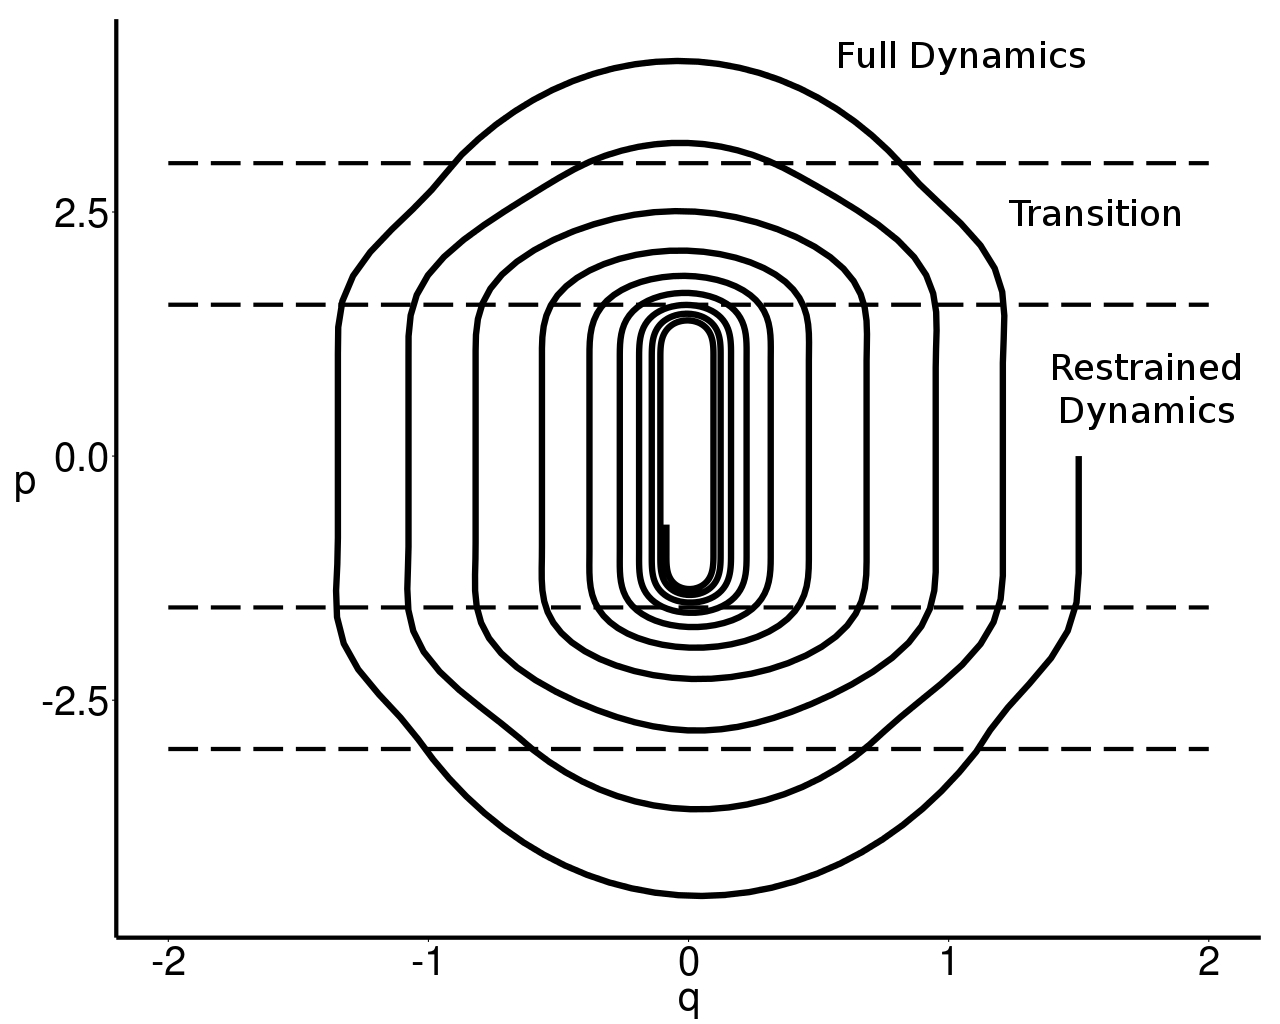
\includegraphics[width=0.8\linewidth]{images/arps-vriphys2013/implicitHOPPraw.jpeg}
  \caption[ARPS: Phase portrait of an implicit ARPS harmonic oscillator]{\label{fig:implicitHOPP} Phase portrait of a harmonic oscillator simulated using implicit ARPS.}
\end{figure}

Figure~\ref{fig:implicitHOPP} shows the phase portrait of a harmonic oscillator simulated using our implicit formulation.
As expected, the well-known numerical damping effect of implicit Euler provides us with the same behavior we could observe with a damped harmonic oscillator.
%%% IMPLICIT HARMONIC OSCILLATOR DAMPED%%%
To include a damping term in the physical model, we derived an implicit formulation which includes a damping term $f_{d} = -\gamma \dot{q}$:
\begin{equation}
	\label{eq:arpsLinearSystemDamped}
	( I + h\gamma M^{-1}R -h^{2}KRM^{-1} ) \Delta p = h( f + h KM^{-1}s + f_{d})
\end{equation}
%------------------------------------------------------------------------
\paragraph*{Solving the equation:}
We exploit inactive particles to save computation time.
As discussed earlier, inactive particles can be handled using explicit integration, which is much simpler.
When a particle is inactive and has no active neighbors we do not need to include it in the linear system.
We thus build the minimal linear system, which only contains active particles and their neighbors.
These particles are implicitly integrated, while the others are explicitly integrated.
\begin{table}[htb]
    \centering
\begin{tabular}{|c|c|c|c|} \hline
    Simulation & Implicit  & Hybrid    & Speed-up \\
    Time & & & \\ \hline
    20s             & 16.9s     & 6.2s      &  \{0.77, 15.16, 2.73\}\\ \hline
\end{tabular}
\caption[ARPS: Implicit vs. Hybrid solver - Measurements]{\label{tab:clothePerf}Implicit solver vs Hybrid solver. Computation time and speedup \{min, max, mean\}.}
\end{table}
Figure~\ref{fig:clothARPS} shows a hanging cloth with active and inactive particles.
At the beginning all the particles become active. Then a moving front of inactivation/reactivation traverses the cloth at decreasing frequency. The cloth finally finds a rest position, where all the particles are inactive and simulated explicitly, saving computation time. The particles can become active again if external forces or imposed motion are applied.
\begin{figure}[htb]
  \centering
  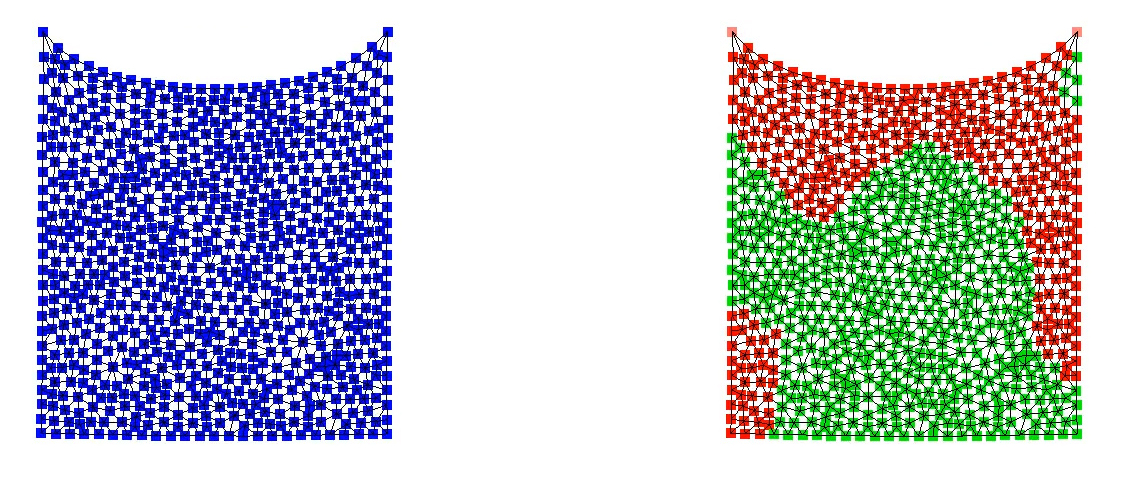
\includegraphics[width=0.8\linewidth]{images/arps-vriphys2013/Square3.jpg}
  \caption[ARPS: ARPS cloth simulation]{\label{fig:clothARPS} Hanging cloth. Left: traditional implicit simulation. Right: implicit ARPS simulation with a varying set of active and inactive particles. }
\end{figure}
Table~\ref{tab:clothePerf} shows performances we achieved with our hybrid solver.
As soon as a large number of particles become inactive the simulation is explicitly integrated and interesting speedup can raise.
\newline
However, while smoothly varying external forces are well handled by our simulator, we noticed instabilities when interacting strongly with the model.
They seem to occur during the transition between the transitive and the full-dynamics states.
A more thorough study of the influence of the transition function $\rho$ on the stability of the system would be necessary to come up with robust implicit ARPS simulations.
 This transition should be really well taken to avoid any instabilities.

\section{Implementation} 
\label{sec:arps_implementation}

\subsection{ Parameters }
ARPS use two parameters, $\epsilon^{r}$ and $\epsilon^{f}$ of Equation~\ref{eq:restrainingfunction}.
The main goal of ARPS in computer graphics is to save time when nothing happens.
So we generally want a low $\epsilon^{r}$ not to miss interesting movements.
When sudden movements occur, we want a normal reaction, so we want the inactive particles to quickly become active.
This requires a short transition, \textit{i.e.} $\epsilon^{f}$ close enough to $\epsilon^{r}$.
However, due to discrete time integration, a short transition may be stepped over, or not enough sampled, which may result in instabilities.
Currently we manually set the parameters, and defer the automatic tuning to future work.
In table \ref{tab:parameters} we refer the thresholds used in our simulations.
\begin{table}[htb]
    \centering
    \begin{tabular}{|c|c|c|c|} \hline
                & $\epsilon^{r}$    & $\epsilon^{f}$ & Tolerance \\ \hline
        SPH     &   1-e6            & 2-e5          & 8e-5 \\ \hline
        Cloth  &   0.05            & 1             & 1e-4 \\ \hline
\end{tabular}
    \caption[ARPS: Parameters for ARPS solver]{\label{tab:parameters} ARPS thresholds for SPH and Cloth simulation}
\end{table}

\subsection{Linear solver}
A linear equation solver is necessary in implicit integration, as presented in Section~\ref{sec:arps_implicit}.
In contrast with most formulations, implicit ARPS generally results in an unsymmetrical equation matrix, due to the matrix products in eq.(\ref{eq:arpsLinearSystem}).
We currently use a sparse LU solver from umfpack library, but it would be interesting to try a Conjugate Gradient method for unsymmetrical matrices to control the computation time, as it is usually done in implicit integration.

%-------------------------------------------------------------------------
\subsection{Choice of the restraining function and criterion}
In ARPS the restraining function is a $5^{th}$-order spline.
The spline directly depends on particle kinetic energy which is the \emph{restraining} criterion.
The implicit solver involves second derivatives of the restraining function, which may have large values, leading to instabilities.
We found that controlling the state of the particles based on momenta norm rather than kinetic energies seems to mitigate this and lead to more stable simulations.
We plan to investigate this issue in future work.


%-------------------------------------------------------------------------
\section{Discussion and concluding remarks} 
\label{sec:arps_discussion}
We have shown that ARPS, a new, simple approach to adaptive simulation, can effectively be applied to Computer Graphics, and we have demonstrated two specific applications.
The most successful one is the SPH simulation, for which we have obtained significant speedups with only minor changes to the original simulation method.
In the case of stiff material, we have obtained promising results for implicit integration, and we will address stability issues in future work, starting with a careful study of the restraining function.

Another interesting avenue is to employ non-physically-based transition criteria. The current one, based on kinetic energy, is well adapted to molecular dynamics simulation. In Computer Graphics, however, we are more interested in visual results. In future work, we thus plan to investigate the tuning of the transition thresholds based on visibility or distance to the camera, to even more focus the computational power where it most contributes to the quality of the result.
